	\documentclass[10pt,oneside]{CBFT_book}
	% Algunos paquetes
	\usepackage{amssymb}
	\usepackage{amsmath}
	\usepackage{graphicx}
% 	\usepackage{libertine}
% 	\usepackage[bold-style=TeX]{unicode-math}
	\usepackage{lipsum}

	\usepackage{natbib}
	\setcitestyle{square}

	\usepackage{polyglossia}
	\setdefaultlanguage{spanish}
	



	\usepackage{CBFT.estilo} % Cargo la hoja de estilo

	% Tipografías
	% \setromanfont[Mapping=tex-text]{Linux Libertine O}
	% \setsansfont[Mapping=tex-text]{DejaVu Sans}
	% \setmonofont[Mapping=tex-text]{DejaVu Sans Mono}

	%===================================================================
	%	DOCUMENTO PROPIAMENTE DICHO
	%===================================================================

\begin{document}




% =================================================================================================
\chapter{Picture de interacción y perturbación dependiente del tiempo}
% =================================================================================================

Estudiaremos perturbaciones dependientes del tiempo 
\[
	H = H_0 + V(t), \qquad H_0 \Ket{n} = E_n \Ket{n} \; (\text{ datos})
\]
donde, no obstante, $\Ket{n}$ no dependiente del tiempo. 
La idea es que hasta $t=0$ no hay potencial $V$ y luego al {\it encenderse} el potencial el estado pasará
a otro
\[
	\Ket{i} \longrightarrow \Ket{j}.
\]

Se estudiarán transiciones entre autoestados del mismo hamiltoniano $H_0$ (que son estacionarios). 
Un autoestado permanece en el tiempo como tal pero con fase oscilante (como veremos).
\notamargen{Esta deducción está diferente de la carpeta, confío en que sea una versión depurada.
Se la analizará en la próxima fase. En la página 75 y 76 en la práctica hay un resumen de toda
la formulación.}
Usamos una representación de interacción y definimos
\[
	\Ket{\alpha,t_0,t}_s = \euler^{-iH/\hbar(t-t_0)}\Ket{\alpha,t_0}_s
\]
\[
	= \euler^{-iH/\hbar(t-t_0)} \euler^{-iV(t)/\hbar(t-t_0)} \Ket{\alpha,t_0}
\]
\[
	= \sum_n \euler^{-iH_0/\hbar \: t} \euler^{-iV(t)/\hbar \: t} \ket{n}\Braket{n|\alpha,t_0}
\]
\[
	= \sum_n \euler^{-iE_n^0/\hbar \: t }\ket{n}\euler^{-iV(t)/\hbar \: t } \Braket{n|\alpha,t_0}	
\]
\[
	\euler^{iH_0/\hbar t}\Ket{\alpha,t_0,t}_s =
	\sum_n  \underbrace{\euler^{-iV(t)/\hbar \: t} \Braket{n|\alpha,t_0}}_{C_n(t)} \ket{n} = \Ket{\alpha,t_0,t}_I	
\]
es decir que se escriben los kets como
\[
	 \Ket{\alpha,t_0,t}_I = \euler^{iH_0/\hbar t}\Ket{\alpha,t_0,t}_s.
\]
Aquí se puede pensar que 
\begin{itemize}
 \item $C_n(t)$ evoluciona por $V(t)$
 \item $\euler^{-iE_n^0 t/\hbar}$ evoluciona por $H_0$
\end{itemize}

Esto introduce la {\it picture} (o representación) de Dirac, también llamada ``de interacción'', en la 
cual los estados evolucionan con $V(t)$.
La siguiente tabla compara con las anteriores [atrasarla porque lo de los operadores aparece después]
\begin{center}
\begin{tabular}{|c|ccc|}
\hline 
& Dirac & Schrödinger & Heinsenberg \\
\hline 
% & &  & \\
estados & evolucionan & evolucionan & fijos \\
$\Ket{\alpha}$ & con $V(t)$ & con $H$ &  \\
\hline
operadores & evolucionan & fijos & evolucionan \\
 & con $H_0$ &  & con $H$ \\
\hline
base & fijos & fijos & evolucionan \\
$\Ket{a'}$ &  &  &  \\
\hline 
% & & & \\
\end{tabular}
\end{center}

\[
	i\hbar \dpar{}{t}\Ket{\alpha,t_0,t}_s = H \Ket{\alpha,t_0,t}_s
\]
\[
	i\hbar \dpar{}{t}\left( \euler^{-iH_0t/\hbar}\Ket{\alpha,t_0,t}_I \right) = 
	H \euler^{-iH_0t/\hbar} \Ket{\alpha,t_0,t}_I
\]
\[
	i\hbar \euler^{-iH_0t/\hbar}\dpar{}{t} \Ket{\alpha,t_0,t}_I = 
	V(t) \euler^{-iH_0t/\hbar} \Ket{\alpha,t_0,t}_I
\]
\[
	i\hbar \dpar{}{t} \Ket{\alpha,t_0,t}_I = V(t) \Ket{\alpha,t_0,t}_I,
\]
que es la ecuación de evolución de los kets, y es equivalente a la ecuación de Schrödinger.

La definición debe verificar asimismo que 
\[
	_s\Braket{\; A_s \;}_s = _I\Braket{\; A_I \;}_I,
\]
lo cual conduce a
\begin{multline*}
	_I\Braket{\alpha,t_0,t|A_I|\alpha,t_0,t}_I = \\
	_s\Braket{\alpha,t_0,t|\euler^{-iH_0t/\hbar}A_I\euler^{iH_0t/\hbar}|\alpha,t_0,t}_s = 
	_s\Braket{\alpha,t_0,t|A_s|\alpha,t_0,t}_s,
\end{multline*}
o bien a que los operadores evolucionan según 
\[
	A_I = \euler^{iH_0t/\hbar}A_s\euler^{-iH_0t/\hbar}
\]
\[
	\dtot{A_I}{t} = \frac{1}{i\hbar}[A_I, H_0]
\]
que es igual que la ecuación de Heisenberg pero con $\hat{H}_0$ en lugar de $H$.
Los kets base permanecen fijos, porque así lo hacen en Schrödinger, en realidad oscila su fase; entonces 
\[
	\Ket{n,t_0,t}_s = \euler^{-iHt/\hbar} \ket{n,t_0}_s
\]
\[
	\Ket{n,t_0,t}_I = \euler^{iH_0t/\hbar} \euler^{-iHt/\hbar} \ket{n,t_0}_s =
	\euler^{-iVt/\hbar} \ket{n,t_0}_s = \euler^{iH_0t/\hbar} \ket{n,t_0}_s
\]
\[
	\Ket{n,t_0,t}_I = \euler^{iE_0t/\hbar} \ket{n,t_0,t}_s
\]
\notamargen{En la carpeta está primero lo de los kets base y luego la ecuación de movimiento 
que acá aparece inmediatamente debajo de la tabla. Aquí habrá que reordenar material.}

Finalmente, resta ver qué le sucede a los coeficientes.

\[
	\Ket{\alpha,t_0,t}_I = \sum_n \Ket{n}\Braket{n|\alpha,t_0,t}_I = \sum_n C_n(t) \Ket{n}
\]
\[
	C_n(t) = \euler^{iVt/\hbar} \Braket{n|\alpha,t_0}_s
\]
\[
	\Braket{n|\alpha,t_0,t}_I = C_m(t)
\]
con $\Ket{n},\ket{m}$ autoestados de $H_0$, le pego un $\Bra{n}$ a la ecuación de evolución de kets,
\[
	i\hbar \dpar{}{t} \Braket{n|\alpha,t_0,t}_I = \Braket{n|V_I(t)|\alpha,t_0,t}_I
\]
\[
	= \sum_m \Braket{n|V_I(t)|m}\Braket{m|\alpha,t_0,t}_I
\]
\[
	i\hbar \dpar{}{t}C_n(t) = \sum_m C_m(t) \Braket{n|V_I(t)|m}
\]
\[
	i\hbar \dpar{}{t}C_n(t) = \sum_m C_m(t) \Braket{n|V_s|m} \euler^{it(E_n-E_m)/\hbar}
\]
\be
	i\hbar \dpar{}{t}C_n(t) = \sum_m C_m(t) V_{nm}(t) \euler^{i\omega_{nm}t}
	\label{solu_sistema}
\ee
donde $V_{nm}(t) \equiv \Braket{n|V(t)|m}$ y $\omega_{nm} \equiv (E_n-E_m)/\hbar$.
Esta es la ecuación que cumplen los coeficientes, donde $|C_n(t)|^2$ es la probabilidad de hallar al sistema 
en el autoestado $\Ket{n}$.
Resolver esto puede ser muy difícil, salvo en los casos en que es tan fácil que no nos
sirve de nada \footnote{Esto es un patrón que se observa a menudo en física teórica.}.
En efecto, la \eqref{soluc_sistema} es un sistema de ecuaciones diferenciales acopladas.
Esto puede ponerse en forma matricial como
\[
	i\hbar \begin{pmatrix}
	\dot{c}_1 \\ \dot{c}_2 \\ ... \\ \dot{c}_N \\
	\end{pmatrix} 
	=
	\begin{pmatrix}
	V_{11} & V_{12}\euler^{i\omega_{12}} & ... \\ 
	V_{21}\euler^{i\omega_{21}} & V_{22} & ... \\ 
	... \\ 
	... \\
	\end{pmatrix}
	\begin{pmatrix}
	c_1 \\ c_2 \\ ... \\ c_N \\
	\end{pmatrix} .
\]


\subsection{Método perturbativo (dependiente del tiempo)}

Pensaremos en una serie perturbativa 
\[
	C_n(t) = C_n(t)^{(0)} + C_n(t)^{(1)}  + C_n(t)^{(2)}  + ...
\]

El evolucionador temporal en la picture de interacción cumple 
\[
	\Ket{\alpha,t_0,t} = U_I(t,t_0)\Ket{\alpha,t_0}_I, \qquad t > t_0
\]
que viene de  
\[
	i\hbar \dtot{}{t} U_I(t,t_0) = V_I(t) U_I(t,t_0)
\]
con $U_I(t_0,t_0)=\mathbb{1}$, la cual resolviendo nos hace llegar a 
\[
	U_I(t,t_0) = \mathbb{1} - \frac{i}{\hbar}\int_{t_0}^{t} V_I(t')U_I(t',t_0) dt'.
\]

Esta ecuación debe proporcionarnos la forma de hallar $U_I$. Se puede usar una iteración sencilla
\[
	U_I(t,t_0) = \mathbb{1} - \frac{i}{\hbar} \int_{t_0}^t \: V_I(t') \left[ 
	\mathbb{1} - \frac{i}{\hbar} \int_{t_0}^t \: V_I(t'') U_I(t'',t_0) dt''
	\right] \: dt',
\]
\[
	U_I(t,t_0) = \mathbb{1} - \frac{i}{\hbar} \int_{t_0}^t \: V_I(t') \left[ 
	\mathbb{1} - \frac{i}{\hbar} \int_{t_0}^t \: V_I(t'') \left(
	\mathbb{1} - \frac{i}{\hbar} \int_{t_0}^t \: V_I(t''') \left\{ ... \right\} dt''
	\right) dt''
	\right] \: dt',
\]
y esto lleva a la serie de Dyson, casi una expresión formal,
\begin{multline*}
	U_I(t,t_0) = \mathbb{1} - \frac{i}{\hbar}\int V_I(t') dt' + \left( -\frac{i}{\hbar} \right)^2\int_{t_0}^t 
	V_I(t') \int_{t_0}^{t'}V_I(t'')dt'' + ...\\ + \left( -\frac{i}{\hbar} \right)^n 
	\int_{t_0}^t dt'\int_{t_0}^{t'}dt''\int_{t_0}^{t''}dt''' ... \int_{t_0}^{t^{n-1}}dt^{n} V_I(t') 
	V_I(t'')...V_I(t^n)	
\end{multline*}
que es una especie de exponencial $ \euler^{T[-i/\hbar \int V(t) dt ]}$.

La serie de Dyson puede verse como un desarrollo perturbativo.

\subsection{Transiciones entre autoestados del hamiltoniano $H_0$}

Veamos el detalle de las transiciones en el formalismo de Dirac.
\[
	\Ket{i,t_0=0,t}_I = U_I(t,0) \Ket{i} = \sum_n \Ket{n}\Braket{n|U_I(t)|i}
\]
y como se viera oportunamente
\[
	\Ket{i,t}_I = \sum_n C_n(t)\Ket{n} = \sum_n \left( \Braket{n|U_I(t)|i} \right) \Ket{n}.
\]
La amplitud de transición será 
\[
	C_n(t) = \Braket{n|U_I(t)|i}
\]
con $\Ket{i},\Ket{n}$ autoestados de $H_0$.
Sea $\tilde{C}_n(t)=\Braket{n|U_s(t)|i}$, donde vemos que $\tilde{C}_n(t)$ y $C_n(t)$ difieren en
una fase, y busquemos una expresión 
\[
	\Ket{\alpha, t_0, t}_I = \euler^{iH_0t/\hbar} \Ket{\alpha, t_0, t}_s
\]
\[ 
	= \euler^{iH_0t/\hbar} U_S(t,t_0)\Ket{\alpha, t_0}_s
\]
\[
	\Ket{\alpha, t_0, t}_I  = \euler^{iH_0t/\hbar} U_S(t,t_0) \euler^{-iH_0t_0/\hbar}  \Ket{\alpha, t_0}_I
	= U_I(t,t_0) \Ket{\alpha,t_0}_I
\]
\[
	\euler^{iH_0t/\hbar} \hat{U}_S \euler^{-iH_0t_0/\hbar} = \hat{U}_I
\]
y notemos que $\hat{U}$ no obedece la ley de transformación de operadores.

\[
	C_n(t) = \Braket{n|\euler^{iH_0t/\hbar} U_S(t,t_0) \euler^{-iH_0t_0/\hbar}|i}
\]
\[
	C_n(t) = \euler^{-i/\hbar[E_n^{(0)} t - E_i^{(0)} t_0]} \Braket{n| U_S(t,t_0) |i} =
		\euler^{-i/\hbar[E_n^{(0)} t - E_i^{(0)} t_0]} \tilde{C}_n(t)
\]
lo que lleva a 
\[
	|C_n(t)|^2 = |\tilde{C}_n(t)|^2.
\]
Para transiciones entre autoestados de $H_0$ los coeficientes dan la misma probabilidad 
(evaluados con el evolucionador de Dirac que con el de Schrödinger).
Debe notarse que esto se cumple siempre y cuando la transición sea entre autoestados del
hamiltoniano y la fase resulte así global.


Veamos las transiciones 
\[
	\Braket{ n | U_I(t,t_0)| i }
\]
a los diferentes órdenes en la perturbación
\begin{itemize}
 \item orden 0
 \[
	C_n^{(0)}(t) = \Braket{n|1|i} = \delta_{ni}
 \]
 \item orden 1
 \[
 	C_n^{(1)}(t) = -\frac{i}{\hbar} \int_{t_0}^t \euler^{i\omega_{ni} t'} V_{ni}(t') dt' \qquad \qquad 
 	V_{ni} \equiv \Braket{n|V(t)|i}
 \]
 \item orden 2
 \[
 	C_n^{(2)}(t) = \sum_m \left( -\frac{i}{\hbar} \right)^2  \int_{0}^t  dt'\int_{0}^t dt''
 	\euler^{it'/\hbar(E_n-E_m)} V_{nm}(t') \euler^{it''/\hbar(E_m-E_i)} V_{mi}(t'')
 \]
\end{itemize}
y entonces la probabilidad de ir desde $\ket{i} \to \Ket{n}$ con $i\neq n$, hasta orden dos, sería
\[
	P^{(2)}_{i\to n} = |C_n^{(0)}(t)+C_n^{(1)}(t)+C_n^{(2)}(t)|^2 =
	| C_n^{(1)}(t) + C_n^{(2)}(t) |^2
\]
donde debe notarse que hay interferencia entre los diversos términos.

\begin{ejemplo}{\bf Sobre observación en práctica}

Había anotado como conclusión en el resumen dado en la práctica que a primer orden solo hay transiciones
entre estados consecutivos. A segundo orden solo hay transiciones hasta el segundo consecutivo (esto se
ve claro en los diagramas de Feynmann).
Luego, aclaré que esto no es cierto en general y que hay que mirar el potencial $V(t)$.
 
\end{ejemplo}

\begin{ejemplo}{\bf Ejercicio 12}

Consideramos el siguiente
\[
	H = H_0 + F_0 x \cos (\omega t), \qquad \qquad 
	H_0 \Ket{n} = \hbar \omega \left( n + \frac 1 2 \right), \Ket{i} = \Ket{0}
\]
con $\Braket{n|V(t)|0} = F_0 \cos(\omega t) \Braket{n|x|0}$. Escribimos $x$ en función de $a,a^\dagger$
con lo cual solamente sobrevive $n=1$
\[
	\Braket{1|V(t)|0} = F_0  \cos(\omega t) \sqrt{ \frac{\hbar}{2 m \omega_0 } }
\]

Tenemos $C_0^{(0)}(t)=1$ y $C_1^{(0)}(t)=0$ que significa que no hay transición cuando estamos en un
autoestado de $H$.
Luego, $C_0^{(1)}(t)=0$ y para 
\[
	C_1^{(1)}(t) = - \frac{i}{\hbar} \int_{t_0}^t \: \euler^{i (E_1 - E_0) t' / \hbar } \:
	\sqrt{ \frac{\hbar}{2 m \omega_0 } } \: F_0 \cos(\omega t') \: dt'
\]
y esto da algo.
Escribo
\[
	\Ket{\psi(t)}_I \approx ( C_0^{(0)} + C_0^{(1)}  ) \Ket{0} + ( C_1^{(0)} + C_1^{(1)} ) \Ket{1}
	= \Ket{0} + C_1^{(0)}(t) \Ket{1}
\]
Este estado no está normalizado porque es una aproximación a orden dado donde no se han tirado los
subsiguientes términos, lo cual está bien porque es una aproximación. Si normalizase otra vez quedo
con un problema diferente. Piden calcular $\vm{x}$.
\[
	\vm{x} = _I\Braket{\psi(t)| \euler^{i H_0 t/\hbar} x \euler^{-i H_0 t/\hbar} |\psi(t)}_I
	= \Braket{\psi(t)| U_I^+ \euler^{i H_0 t/\hbar} x \euler^{-i H_0 t/\hbar} U_I |0}
\]
Resulta
\[
	C_1^{0} = \frac{i F_0 }{\sqrt{ 2 \hbar m \omega_0 } (\omega - \omega_0)}
\]
y si $\omega - \omega_0$ es cercano a cero me alejo demasiado de la normalización del estado y entonces
en realidad no tiene mucho sentido el método perturbativo.
Vale con coeficientes pequeños: si los coeficientes son grandes estaré tirando una cosa de norma grande
y no tiene sentido.

\end{ejemplo}


\subsection{Ejemplo: potencial constante encendido abruptamente}

Sea un potencial que prendemos y apagamos luego, pero constante. Es decir
\[
	V(t) = \begin{cases}
	0 	& t < 0  \\
	V(r,p,s,L,...) & t \geq 0
	\end{cases}
\]
donde $V \neq V(t)$, pero puede depender de cualquier otra cosa. La figurilla más abajo
ilustra este {\it escalón}.

\includegraphics[width=0.45\textwidth]{images/teo2_22.pdf}

A orden cero no vemos cambio pues
\[
	C^0_n(t) = 0.
\]
A orden uno es 
\[
	C^1_n(t) = -\frac{i}{\hbar} \int_0^t \euler^{i/\hbar(E_n - E_i)t'} V_{ni} \: dt'=
	\frac{V_{ni}}{(E_n - E_i)}(1-\euler^{i\omega_{ni}t})
\]
donde debemos notar que si esto revienta porque $E_n \sim E_i$ entonces la teoría de
perturbaciones no puede usarse aquí.

Evaluando la probabilidad se tiene	
\[
	|C^1_n(t)|^2 = 
	\frac{4|V_{ni}|^2}{| E_n - E_i|^2}\sin^2\left(\frac{(E_n - E_i)t}{2\hbar}\right).
\]

	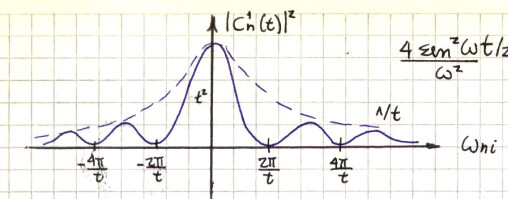
\includegraphics[width=0.45\textwidth]{images/fig_ft2_potencial_abrupto.jpg}

Es máxima la probabilidad cuando $\Delta E\to 0$. 
En ese caso las transiciones son a estados de la misma energía. 
El gráfico de arriba es a un dado $t$ fijo. A medida que el tiempo transcurre el gráfico
tiende a una delta de Dirac.

A tiempo largo la probabilidad es no nula para aquellos estados 
\[
	t \sim \frac{2\pi}{|\omega_{ni}|}
\]

Hay probababilidad de transición $\Ket{i} \to \Ket{n}$ apreciable donde $\omega = \frac{2\pi}{t}
= \frac{\Delta E}{\hbar}$ dado que $\Delta t \Delta E \sim \hbar $. O bien, $\Delta E \sim 0$.

\section{Scattering}

Podemos pensarlo como el caso de un potencial que se prende y apaga, representando éste el objeto
contra el cual se hace scattering.

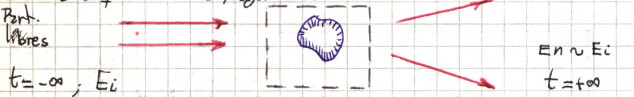
\includegraphics[width=0.6\textwidth]{images/fig_ft2_scattering_intro.jpg}

Este último ejemplo puede aplicarse a colisiones elásticas. Prendemos y apagamos un potencial que es el 
masacote al cual impactamos. De entrada ha partículas libres y de salida (lejos de $V$) partículas libres.
Entonces $ E_n - E_c \sim 0$ y consideraremos lo que sucede a tiempos largos. Interesará la probabilidad 
total de transicionear a estados de energía similares a $E_i$. Por ello se considera 
\be
	\sum_{\substack{n \\ E_n\sim E_i}} |C^1_n(t)|^2 
	\longrightarrow 
	\int \: \rho(E_n) \: |C^1_n(t)|^2 \: dE_n
	\label{scattering_integral}
\ee
donde el integrando es el número de estados dentro de un intervalo de energías $(E,E+dE)$ a los cuales
se puede transicionar. Esta erá la probabilidad de transición.

\begin{figure}[htb]
	\begin{center}
	\includegraphics[width=0.6\textwidth]{images/teo2_23.pdf}
	\end{center}
	\caption{}
\end{figure} 

A primer orden la probabilidad será algo como
\[
	\lim_{t\to\infty} \; \int \: \rho(E_n) \: \frac{4|V_{ni}|^2}{| E_n - E_i|^2}
	\sin^2\left(\frac{(E_n - E_i)t}{2\hbar}\right) \: dE_n,
\]
puesto que estamos considerando lo que sucede a tiempos muy largos.
En esos casos, como la probabilidad tiende a una delta de Dirac, 
\[
	\lim_{t\to\infty} \frac{1}{| E_n - E_i|^2}
	\sin^2\left(\frac{(E_n - E_i)t}{2\hbar}\right) = \frac{\pi t}{2\hbar} \delta(E_n - E_i),
\]
la integración es fácil y se obtiene
\[
	\lim_{t\to\infty} \; \int \: \rho(E_n) |C^1_n(t)|^2 \: dE = 
	\left.\left(\frac{2\pi}{\hbar}\right) \rho(E_n) |\bar{V}_{ni}|^2 \: t \: \right|_{E_n\sim E_i}
\]
donde $\bar{V}_{ni}$ es un potencial promedio. La probabilidad de transición es proporcional a $t$. 

Se suele definir una tasa de transición (probabilidad de transición por unidad de tiempo)
\[
	\dtot{}{t}\left( \sum_{\substack{n \\ E_n\sim E_i}} |C_n^{(1)}|^2 \right) =
	\left(\frac{2\pi}{\hbar}\right)	|\bar{V}_{ni}|^2 \rho(E_n) = \omega_{i\to n}^{(1)}
\]
que es la regla de oro de Fermi, y sirve para calcular cualquier transición entre estados
para potenciales que no dependen del tiempo.

[reacomodar]
La energía al final se mide con cierto error $\Delta E$ de modo que se obtendrá $E \pm \Delta E$ y 
deberá sumar [no sé bien qué se quiere decir acá]
\[
	\sum_n | C_n(t) |^2 \quad (E_n \sim E \pm \Delta E)
\]
Pero si no es discreto necesitaré integrar (la integral \eqref{scattering_integral})

\section{El método variacional}

Se puede usar para aproximar la energía del estado fundamental (el estado de energía mínima).
No conocemos $\Ket{n}$ ni $E_n$, pero $ H \Ket{n} = E_n \Ket{n}$ donde $\{ \Ket{n} \}$ es
una base.
Evaluamos
\[
	\Braket{\psi|H|\psi} = \sum_{n,m}\Braket{\psi|n}\Braket{n|H|m}\Braket{m|\psi} =
		\sum_{n,m} E_n \Braket{\psi|n}\Braket{n|m}\Braket{m|\psi} 
\]
\[
	\Braket{\psi|H|\psi} = \sum_{n,m} E_n C_n^*\Braket{n|m}C_m = \sum_{n} E_n|C_n|^2
\]
\[
	\sum_{n} E_n|C_n|^2 \geq \sum_n E_0|C_n|^2 = E_0 \sum_n |C_n|^2 = E_0 \Braket{\psi_n|\psi_n}
\]
y usamos 
\[
\Ket{\psi} = \sum_n \Braket{n|\psi}\Ket{n} \qquad \Bra{\psi} = \sum_n \Braket{\psi|n}\Bra{n} 
\]
para arribar a
\[
	\frac{\Braket{\psi_n|H|\psi_n}}{\Braket{\psi_n|\psi_n}} \geq E_0.
\]
donde $E_0$ es la energía más baja. Esto no parece ser muy iluminador que digamos.
Se considera que $\psi$ es tal que 
\[
	\Braket{x|\psi} = \psi(x)_{|x|\to\infty} \to 0
\]
lo que significa que la función de onda es {\it well behaved} (bien comportada).

\begin{ejemplo}{\bf Ejercicio 10}

A partir de $ \Braket{x|\psi} = \euler^{-\b|x|}$ se tiene, intercalando la completitud,
\[
	\Braket{\psi|\psi} = 
	\int_{-\infty}^\infty \: \Braket{\psi | x'}\Braket{x' | \psi} \: dx' = 
	2 \int_{-\infty}^\infty \: \euler^{- 2 \b |x| } \: dx = \frac{1}{\b}
\]
y del mismo modo
\begin{multline*}
	\Braket{\psi|H|\psi} = \Braket{\psi| \frac{p^2}{2 m} + \frac{m \omega^2 x^2 }{2} |\psi} = \\
	- \Frac{\hbar^2}{2m} \int_{-\infty}^\infty \: 
	\dtot[2]{}{x}\left( \Braket{\psi|x} \right)\Braket{x'|\psi} \: dx' +
	\frac{m\omega^2}{2} \int_{-\infty}^\infty \: \Braket{\psi|x^2|x'} \Braket{x'|\psi} \: dx',
\end{multline*}
para finalmente
\[
	\Braket{\psi|H|\psi} = - \Frac{\hbar^2}{2m} \int_{-\infty}^\infty \: 
	\dtot[2]{}{x}\left( \euler^{- \b |x| } \right) \euler^{- \b |x| } \: dx' +
	\frac{m\omega^2}{2} \int_{-\infty}^\infty \: \euler^{- 2 \b |x| } x^2 \: dx'
\]

Trabajaremos por partes esta cosa. Una integral con la doble derivada se convierte en
\[
	\int_{-\infty}^\infty \: u \dtot[2]{u}{x} \: dx = 
	\left. u \: \dtot{u}{x} \right|_{-\infty}^\infty - \int_{-\infty}^\infty \: \Dtot{u}{x}^2 \: dx
\]
donde el primer término es nulo porque la función de onda es bien comportada.
Con este enfoque resulta
\[
	\Braket{\psi|H|\psi} = - \frac{\hbar^2 \b}{2m} + \frac{m\omega^2}{4\b^3},
\]
y entonces \notamargen{Typo seguro.}
\[
	\mathcal{E}(\psi) = \b \left( - \frac{\hbar^2 \b}{2m} + \frac{m\omega^2}{4\b} \right) \geq E_0 
\]
y entonces desde
\[
	\left. \dpar{\mathcal E}{\b}\right|_{\b_{\text{min}}} = 0
\]

El único parámetro libre es $\b$; entonces se calcula el $\beta$ que hace minimo esta cosa y ya está
resuelto.
 
\end{ejemplo}

\begin{ejemplo}{\bf Ejercicio 11}

Tenemos la siguiente ecuación:
\[
	\dtot[2]{\psi}{x} + (\lambda -|x|)\psi = 0,
\]
con $\psi \to 0$ si $|x|\to\infty$. Se tiene
\[
	\begin{cases}
	 C(\a - |x|) & |x|\leq \a \\
	 0 & |x| > \a
	\end{cases}
\]

Para el hamiltoniano en cuestión es
\[
	\left[ \right] \Ket{\psi} = \mathcal E \Ket{\psi},
\]
que conduce a la ecuación
\[
	- \frac{\hbar^2}{2m} \dtot[2]{\psi}{x} + V(x)\psi = \mathcal E  \psi
\]
la cual reescribimos como
\[
	\dtot[2]{\psi}{x} + 
	\left[ \frac{2m}{\hbar^2} \mathcal E - \frac{2m}{\hbar^2} V(x) \right] \psi  = 0
\]
e identificamos a ojo que
\[
	V(x) = \frac{\hbar^2}{2m}|x|, \qquad \lambda = \frac{2m\mathcal E}{\hbar^2}
\]
de manera que habría que minimizar $\lambda$ haciendo mínimo $\mathcal E$ respecto de $\a$.
 
\end{ejemplo}

\begin{ejemplo}{\bf Ejercicio 7}

Estamos en el átomo de hidrógeno. Es decir $\Ket{n,\ell,m}$ donde $n \in \mathbb N$, $\ell < n$
y $-\ell \leq m \leq \ell$.

Tendremos
\begin{eqnarray*}
 n=1 \qquad & \Ket{1 0 0 } \\
 n=2 \qquad & \Ket{211}, \Ket{210}, \Ket{21-1}, \Ket{200}
\end{eqnarray*}
donde los primeros tres del orden dos son $\Ket{2p} = \Ket{21m}$ y el último es $\Ket{2s}$.
La perturbación requerirá una matriz de $5\times5$ y habrá que diagonalizar $E_2^{(1)}$, que
es el bloque inferior (ver iluscración).
La perturbación es algo del tipo $V = - e E z $

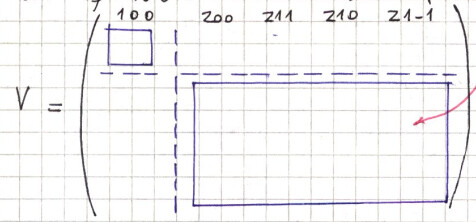
\includegraphics[width=0.5\textwidth]{images/fig_ft2_ejercicio7A.jpg}

Tenemos
\[
	\Braket{2 \ell m|-eEz|2\ell' m'} = -e E \Braket{2\ell m|z|2\ell' m'}
\]
y como el operador paridad cumple $\Pi z \Pi^{-1} = -z$ se da
\[
	\Pi \Ket{n\ell m} = (-1)^\ell \Ket{n\ell m}
\]
lo cual no es otra cosa que usar reglas de selección. Luego,
\[
	\Braket{2\ell m|-z|2\ell' m'} = (-1)^{\ell+\ell'} \Braket{2\ell m|z|2\ell' m'}
\]
y si $\ell+\ell'=L$ entonces el braket es nulo y sobreviven $\ell\neq \ell'$ de modo que
$\Braket{21m|z|200}$ es el que permanece.

Por Wigner-Eckart $z=T_0^1$ de modo que
\[
	\Braket{\a' j' m'|T_q^k|\a j m} = И \Braket{j k m q|j k j' m'}
\]
donde $И$ es una constante. Entonces
\[
	\Braket{21m|T_0^1|200} = И \Braket{0100 | 011m }
\]
desde lo cual sobreviven $\Braket{0100|011m}$ si $m=0$.

Entonces se tiene lo que ilustra la imagen

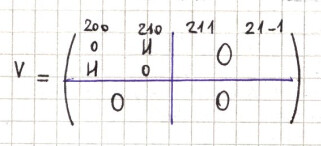
\includegraphics[width=0.5\textwidth]{images/fig_ft2_ejercicio7B.jpg}

y como es una matriz de Pauli su diagonalización es un juego de niños. Se tienen
\[
	\Ket{v_1} = \frac{1}{\sqrt{2}} \left( \Ket{200} + \Ket{210} \right)
	\qquad \qquad 
	\Ket{v_2} = \frac{1}{\sqrt{2}} \left( \Ket{200} - \Ket{210} \right)
\]

Si se cambia de base y se escribe el potencial $V$ en la base $\{ \Ket{100}, \Ket{v_1}, 
\Ket{v_2}, \Ket{211}, \Ket{21-1} \}$ se tiene

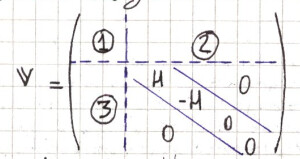
\includegraphics[width=0.5\textwidth]{images/fig_ft2_ejercicio7C.jpg}

que es una matriz diagonal por bloques. 
 
\end{ejemplo}

\subsection{Scattering a orden dos y OFPT}

Para el coeficiente a orden 1 teníamos la regla de oro de Fermi.
El coeficiente a orden dos es
\[
	C_n^{(2)} = \Frac{-i}{\hbar}^2 \sum_{m \neq i} V_{nm} V_{mi}
	\int_0^t \: dt' \: \euler^{ i \omega_{nm} t'} 
	\int_0^{t'} \: dt'' \: \euler^{ i \omega_{ni} t''}
\]
donde la integral más interna se aproxima como
\[
	\frac{i}{\omega_{mi}} \left[ 1 - \euler^{ i t' \omega_{mi} } \right]
\]
y eso nos permite considerar el siguiente límite
\[
	\lim_{t \to \infty} C_n^{(2)} = 
	\frac{i}{\hbar} \: \sum_{m \neq i} \: \frac{V_{nm} V_{mi}}{E_n - E_i}
	\int_0^t \: dt' \: ( \euler^{ i \omega_{ni} t'} - \euler^{ i \omega_{nm} t'} ),
\]
de manera que a orden dos es
\[
	\omega_{i\to n}^{(2)} = \frac{2\pi}{\hbar}\left. \left| \overline{ V_{ni} + \sum_{m\neq i} 
	\frac{V_{nm}V_{mi}}{(E_i-E_m)}} \right|^2 \rho(E_n) \right|_{E_n\sim E_i}.
\]

Para obtener los siguientes términos dentro del $\bar{||^2}$ podemos emplear un ardid gráfico conocido como 
{\it Old Fashioned Perturbation Theory}, que no es más que un artilugio diagramático mnemotécnico.

Consideramos un caso como el scattering de una zona donde existe un potencial al que bombardeamos con
partículas en estados $\Ket{i}$ y que salen partículas con estados $\Ket{n}$ de la misma energía.
Ver figura inicial en Fig siguiente.

\includegraphics[width=1.0\textwidth]{images/teo2_24.pdf}

Luego, el estado $\Ket{m}$ es un pseudoestado virtual que no conserva la energía y es un artificio surgido
del cálculo (ver figura intermedia). El segmento entre los vértices es un {\it propagador} y de alguna manera
podemos hacernos la idea de que transporta la perturbación entre vértices. Cada uno de los vértices es
un elemento de matriz.

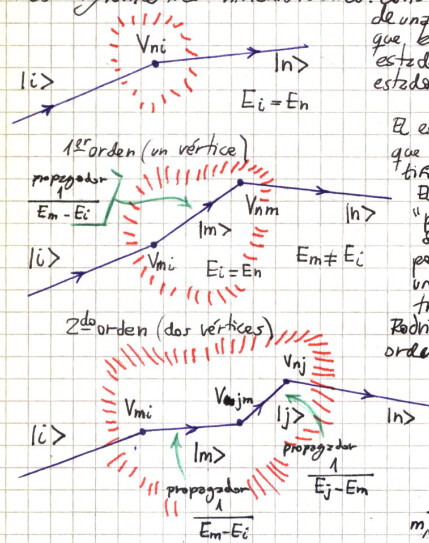
\includegraphics[width=0.6\textwidth]{images/fig_ft2_tre_ordenes_perturbativos.jpg}

Podríamos avanzar con este grafismo y especular con lo que sucede a tercer orden. Este término será sumar
sobre todos los caminos posibles
\[
	\sum_{m,j \neq i, m \neq j} V_{nj} \frac{1}{E_j - E_m} 
	V_{jm} \frac{1}{E_m - E_i} V_{mi}.
\]

Estos diagramas son los que llevan el nombre de OFPT. Es importante notar que implica que entre los
estados intermedios estados virtuales $\Ket{m},\Ket{j}$ no se conserva la energía; son propagadores.
La energía se conserva solo en el inicial y el final. Si la energía se conservase reventarían los
denominadores.

Consideremos ahora una perturbación armónica dada en términos de un potencial escrito de forma
hermítica
\[
	V(t) = \mathbb{V} \euler^{i\omega t} + \mathbb{V}^\dagger \euler^{-i\omega t},
		\qquad \mathbb{V}\neq \mathbb{V}(t)
\]
Encendemos este potencial y queremos pasar de estados $\Ket{i} \to \Ket{n}$ viendo su probabilidad de 
transición a orden uno,
\[
	C_n^{(1)}(t) = -\frac{i}{\hbar} 
	\int_0^t ( V_{ni}\euler^{i\omega t'}+ V_{ni}^\dagger \euler^{-i\omega t'} )
	\euler^{i\omega_{ni}t'}dt'
\]
donde la diferencia con un potencial constante es el primer término del paréntesis [?]. Entonces,
\[
	C_n^{(1)}(t) = -\frac{i}{\hbar} \left[ V_{ni} \int_0^t \euler^{i(\omega +\omega_{ni})t'} dt' + 
		V_{ni}^\dagger \int_0^t \euler^{i(-\omega +\omega_{ni})t'} dt' \right]
\]
\[
	C_n^{(1)}(t) = -\frac{i}{\hbar} \left[ V_{ni} 
	\frac{\euler^{i(\omega +\omega_{ni})t} -1}{i( \omega +\omega_{ni} )}
	+ V_{ni}^\dagger \frac{\euler^{i(-\omega +\omega_{ni})t} - 1}{i(-\omega +\omega_{ni})} \right]
\]
\[
	C_n^{(1)}(t) = \frac{V_{ni}}{\hbar} \frac{1-\euler^{i(\omega +\omega_{ni})t}}{( \omega +\omega_{ni} )}
	+ \frac{V_{ni}^\dagger}{\hbar} \frac{1-\euler^{i(-\omega +\omega_{ni})t}}{(-\omega +\omega_{ni})}
\]
donde se ve que el primer término es similar a $\delta(\omega_{ni} +\omega)$ y el segundo a
$\delta(\omega_{ni} - \omega)$ de suerte que
\[
	\lim_{t\to\infty} C_n^{(1)}(t) = \frac{1}{\hbar}\left[ V_{ni}\delta(\omega_{ni}+\omega) 
		+ V_{ni}^\dagger \delta(\omega_{ni}-\omega) \right]
\]
Esto representa $E_n = E_i - \hbar \omega$ en el primer término y $E_n = E_i + \hbar \omega$ en el segundo
que pueden asociarse a la emisión de un cuanto de energía en la interacción o a la absorción, respectivamente.

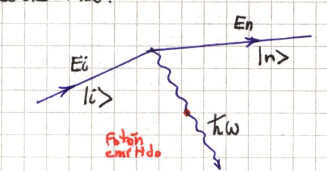
\includegraphics[width=0.4\textwidth]{images/fig_ft2_perturbativos_1a.jpg}
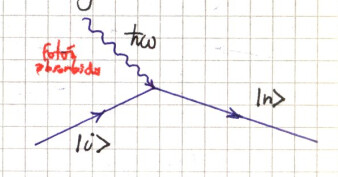
\includegraphics[width=0.4\textwidth]{images/fig_ft2_perturbativos_1b.jpg}

Entonces todo el término representa la probabilidad de emitir o absorber fotones.
Veamos el ejemplo de emisión o absorción que ocurre en un átomo.

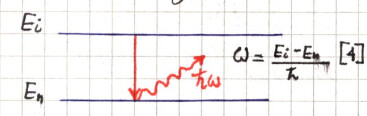
\includegraphics[width=0.4\textwidth]{images/fig_ft2_perturbativos_2a.jpg}
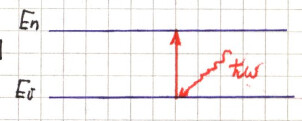
\includegraphics[width=0.4\textwidth]{images/fig_ft2_perturbativos_2b.jpg}

Los $V,V^\dagger$ se puede asociar como que aniquilan o crean fotones.
Otro asunto es que al descomponer un campo EM en Fourier tengo las frecuencias $\omega$ separadas
y debería sumar entre todas las frecuencias, pero se ve que no es necesario y la única que debo
considerar es [4] (número dentro de la figura!).

Luego será nulo sólo si 
\[
	\omega_{ni} = -\omega \qquad \longrightarrow \qquad 
		\frac{E_n - E_i}{\hbar} = -\omega \quad E_n = E_i - \hbar\omega
\]
\[
	\omega_{ni} = -\omega \qquad \longrightarrow \qquad 
		\frac{E_n - E_i}{\hbar} = \omega \quad E_n = E_i + \hbar\omega
\]

\begin{figure}[htb]
	\begin{center}
	\includegraphics[width=1.0\textwidth]{images/teo2_25.pdf}
	\end{center}
	\caption{}
\end{figure} 

Luego, $ \lim_{t\to\infty} C_n^{(1)}(t) $ representa la probababilidad de emitir o absorber 
fotones en una interacción. Se puede asociar que $V$ crea fotones y $V^\dagger$ destruye fotones. 
Para un átomo se tiene 

\begin{figure}[htb]
	\begin{center}
	\includegraphics[width=1.0\textwidth]{images/teo2_26.pdf}
	\end{center}
	\caption{}
\end{figure} 

En teoría de perturbaciones de dos partículas vemos que a orden $n$ se intercambian $n$ fotones.

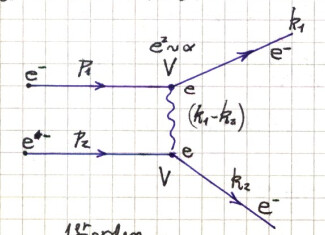
\includegraphics[width=0.4\textwidth]{images/fig_ft2_perturbativos_3a.jpg}
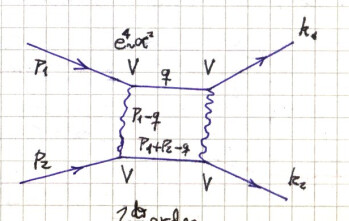
\includegraphics[width=0.4\textwidth]{images/fig_ft2_perturbativos_3b.jpg}

En el gráfico de la izquierda a primer orden los impulsos están determinados mientras que a orden
dos, en el gráfico de la derecha, no sabemos el impulso $q$ y debiéramos integrar pero la integral
da infinito
\[
	\lim_{\Lambda \to \infty} \int_{-\Lambda}^\Lambda \: dq.
\]
Feymann desarrolló una ``renormalización'' que tapa estos infinitos considerando que hay que usar
una serie perturbativa para la carga $e$ en los vértices.

Todo este formalismo permite la aparición de partículas y antipartículas. Aquí $\Delta t = t_2 - t_1$ es
tan chico que 
\[
	\Delta t \Delta E \sim \hbar
\]

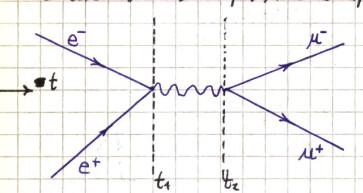
\includegraphics[width=0.4\textwidth]{images/fig_ft2_desdoblamiento_1a.jpg}

La joda es que la ``cosa de abajo'' 

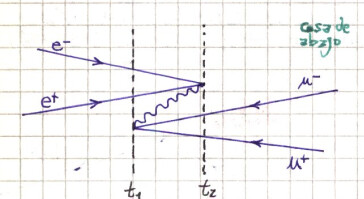
\includegraphics[width=0.4\textwidth]{images/fig_ft2_desdoblamiento_1b.jpg}

es equivalente pero podemos sumarlo para obtener

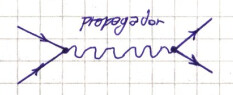
\includegraphics[width=0.4\textwidth]{images/fig_ft2_desdoblamiento_2a.jpg}

que es ocurrencia de Feynmann, pero el propagador es un fotón virtual y puede tener masa.

Este formalismo se puede aplicar directamente también al electromagnetismo. Sea una corriente $j^\mu(x,t)$
que genera un potencial $A^\mu$; se puede calcular con un ``propagador''
\[
	A^\mu(x',t') = \int dx dt \: G^\mu(x,t ; x', t') j^\mu(x,t)
\]
donde la función de Green oficia de propagador para llevar la interacción de $x',t'$ a $x,t$.
Luego, $j_{2\mu}(x',t') A^\mu(x',t')$ es proporcional a la fuerza entre corrientes.
\[
	\int dx dt \: j_{2\mu}(x,t) G^\mu_\nu(x,t ; x', t') j^\nu_1(x,t)
\]

Podemos pensar en un diagramita donde a primer orden se intercambia un fotón

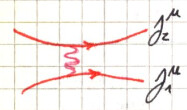
\includegraphics[width=0.3\textwidth]{images/fig_ft2_desdoblamiento_2b.jpg}

\subsection{Despoblamiento de estados iniciales}

Suponemos que pasamos entre estados $\Ket{i} \to \Ket{i}$ (número de estados).
Queremos ver con qué velocidad $v$ se despoblan los $\Ket{i}$. 
Para elllo me construyo un potencial {\it suave}
\[
	\lim_{\eta\to 0} V(t) = \euler^{\eta t} \mathbb{V}, \qquad  \mathbb{V} \; \text{ cte.}
\]
donde $\eta$ es un parámetro regularizador, cuyo fin es regularizar divergencias que
puedan aparecer en el denominador.

\begin{figure}[htb]
	\begin{center}
	\includegraphics[width=0.5\textwidth]{images/teo2_27.pdf}
	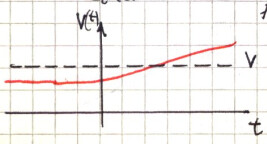
\includegraphics[width=0.4\textwidth]{images/fig_ft2_desdoblamiento_3.jpg}
	\end{center}
	\caption{}
\end{figure} 

Partamos de $ \Ket{i} \to \Ket{n} $
\[
	C_n^{(1)}(t) = \lim_{t\to\infty} -\frac{i}{\hbar} 
	\int_{t_0}^t V_{ni} \euler^{\eta t'} \euler^{i\omega_{ni} t'} dt' =
	-\frac{i}{\hbar} V_{ni} 
	\frac{\euler^{\eta t} \euler^{i\omega_{ni} t} }{\eta+i\omega_{ni}}
\]
y consecuentemente
\[
 	|C_n^{(1)}(t)|^2 = \frac{|V_{ni}|^2}{\hbar^2} 
 	\frac{\euler^{2\eta t} }{\eta^2 + \omega_{ni}^2 }.
\]
La variación temporal será
\[
	\dtot{}{t}|C_n^{(1)}(t)|^2 = 2 \eta \frac{|V_{ni}|^2}{\hbar^2} \frac{\euler^{2\eta t} }{\eta^2 + \omega_{ni}^2 }
\]
y tomando el límite $\eta \to 0$ 
\[
	\lim_{\eta\to 0} \dtot{}{t}|C_n^{(1)}(t)|^2 = 2 \frac{|V_{ni}|^2}{\hbar^2} 
			\frac{\eta }{\eta^2 + \omega_{ni}^2 } = \begin{cases}
	                    0 \quad \text{si}\;\; \omega_{ni}^2 \neq 0 \\
	                    \infty \quad \text{si}\;\; \omega_{ni}^2 = 0
	                   \end{cases}
\]
y llegamos a la regla de oro de Fermi,
\[
	\dtot{}{t}|C_n^{(1)}(t)|^2 = 2 \frac{|V_{ni}|^2}{\hbar^2} \delta(\omega_{ni}) \pi.
\]

Veamos ahora qué sucede cuando $n=i$. Se tienen $C_i^{(0)}(t) = 1$ y [?]
\[
	C_i^{(0)}(t) = - \frac{i}{\hbar} \lim_{t_0 \to -\infty}
	\int_{t_0}^t \: V_{ii} \euler^{\eta t '} dt' = -\frac{ i }{\hbar \eta } V_{ii}\euler^{\eta t}
\]
\[
	C_i^{(2)}(t) = \Frac{-i}{\hbar}^2 \sum_m |V_mi|^2 \lim_{t_0\to\infty}
	\int_{t_0}^t \: dt' \: \euler^{i \omega_{im} t' + \eta t' }
	\frac{\euler^{i \omega_{mi} t' + \eta t' }}{ i ( \omega_{mi} - i \eta ) }
\]
mientras que si dividimos la sumatoria en $m$ se tiene ahora
\[
	= \left( -\frac{i}{\hbar} \right)^2 \frac{|V_{ii}|^2 \euler^{2\eta t}}{2\eta^2}
	- \frac{i}{\hbar} \sum_{m\neq i} \frac{|V_{mi}|^2 \euler^{2 \eta t}}{ 2 \eta ( E_i - E_n + i \hbar \eta ) }
\]

Hasta orden dos tenemos
\[
	C_i(t) = C_i^{(0)}(t) + C_i^{(1)}(t) + C_i^{(2)}(t)
\]
y
\[
	\frac{1}{C_i(t)} \dtot{C_i(t)}{t} = 
	\frac{ 
	-\frac{i}{\hbar} V_{ii} 
	+ \left( -\frac{i}{\hbar} \right)^2 \frac{|V_{ii}|^2 \euler^{\eta t}}{\eta}
	- \frac{i}{\hbar} \sum_{m\neq i} \frac{|V_{mi}|^2 \euler^{2 \eta t}}{E_i - E_n + i \hbar \eta }
	}
	{
	1 - \frac{i}{\hbar \eta} V_{ii} \euler^{\eta t} + C_i^{(2)}(t)
	}
\]
\notamargen{Acá usamos un Taylor para dividir por $1+e$ y así multiplicar por $1-e$... Taylor, pelotudo.}
pero no necesito poner el $C_i^{(2)}(t)$ puesto que al hacer el cociente me generarán términos
cúbicos que tiraré; por ello no lo considero.
Haciendo la cuenta a segundo orden en teoría de perturbaciones de $\eta \to 0$ obtenemos un
límite finito. Tendiendo
\[
	\frac{1}{C_i(t)} \dtot{C_i(t)}{t} = -\frac{i}{\hbar}
	\left[ 
	V_{ii} + \sum_{m\neq i} \frac{|V|^2}{E_i - E_n + i \hbar \eta }
	\right] = -\frac{i}{\hbar} \Delta_i
\]
que implica la ecuación diferencial 
\[
	\dtot{C_i(t)}{t} = - \frac{i}{\hbar} \Delta_i C_i(t)
\]
cuya solución es por supuesto $ C_i(t) = \euler^{- i \Delta_t t / \hbar } $.
Ahora se tiene que la evolución temporal lleva 
\[
	\Ket{i} \longrightarrow C_i(t) \euler^{-i E_i t /\hbar} \ket{i} = 
	\euler^{i (E_i -\Delta i) t / \hbar } \Ket{i}
\]
mientras que a primer orden $ E_i \to E_i + V_{ii}$.

Analicemos el término
\[
	\frac{1}{E_i - E_n + i \hbar \eta}
\]
teniendo en cuenta que en análisis complejo se sulen separar 
\[
	\lim_{\epsilon \to 0 } \frac{1}{x + i  \epsilon} = P_p\left[ \frac{1}{x}\right] - i \pi \delta(x)
\]
y luego, la
\[
	\sum_{m\neq i} \frac{|V|^2}{E_i - E_n + i \hbar \eta }
\]
se descompondrá en una parte real y en una imaginaria, donde esta última representará la difusión con
el tiempo que cobrará importancia si $ E_i = E_n $ y entonces
\[
	C_i^{(2)}(t) = \euler^{- i/\hbar \mathfrak{Re}(\Delta_i) t  + 1/\hbar \mathfrak{Im}(\Delta_i) t}
\]

Se suelen definir el ancho de decaimiento
\[
	\frac{\Gamma_i}{\hbar} = - \frac{2}{\hbar}\mathfrak{Im}(\Delta_i)
\]
de modo que
\[
	|C_i^{(2)}(t)|^2 = \euler^{ - \Gamma_r t /\hbar} = \euler^{ - t/\tau_i}
\]
donde $\tau_i = \hbar / \Gamma_i$. La componente compleja da el decaimiento, como en electromagnetismo,
y también da información de la variación del número de estados $\Ket{i}$

\section{Scattering sección eficaz}

Emplearemos teoría de perturbaciones para hacer este cálculo; aunque este no fue el enfoque histórico original.
Consideraremos el siguiente esquema:

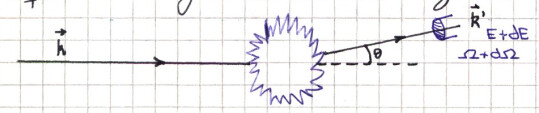
\includegraphics[width=0.5\textwidth]{images/fig_ft2_scattering_section.jpg}

\notamargen{Este tema está muy bien desarrollado en el libro de Sakurai.}
El potencial trabaja en una zona limitada al origen y destino de las partículas bombardeantes consideramos que
son partículas libres.

En el caso más sencillo el potencial es de manera definido como para que las bombardeantes no le transfieren
impulso $\vb k$. Tendremos conservación de la energía.
Entonces, $\Ket{k},\Ket{k}'$ son autoestados de momento (partículas libres), y consideramos
\[
	|\vb{k}| = |\vb{k}'|, 
\]
de que se conserva la energía. 

Consideraremos la aproximación al orden más bajo (aproximación de Born).
La picture es 
\[
	\Ket{\vb k} \longrightarrow \Ket{\vb k'}
\]
\[
	\omega_{\Ket{\vb k} \longrightarrow \Ket{\vb k'}} =
	\int \frac{2\pi}{\hbar} \delta( E_f - E_i ) |\Braket{\vb k'|V|\vb k}|^2 \rho(E_f) dE_f
\]

\begin{figure}[htb]
	\begin{center}
	\includegraphics[width=0.5\textwidth]{images/teo2_28.pdf}
	
	\end{center}
	\caption{}
\end{figure} 

Querríamos calcular en 3E y con extensión infinita la densidad de estados con energía entre $E +dE$.
\[
	\omega = \int \frac{2\pi}{\hbar}  \delta(E'-E) |\Braket{\vb{k}'|V|\vb{k}}|^2 \rho(E') dE'
\]
queremos calcular la densidad de estados de energía entre $(E,E+dE)$. 
Simplificamos pensando en $1D$. Pensamos en una partícula libre en una caja $1D$ de longitud $L$, que
luego haremos tender a infinito.
\[
	N \euler^{i k_x x /\hbar}, \qquad \text{con} \;\; k_x = \frac{2\pi}{L}n_x
\]
pidiendo normalización unitaria $\Braket{k|k}=1$ se tiene 
\[
	\frac{1}{\sqrt{L}} \euler^{i k_x x /\hbar}
\]
con $L\to\pm\infty$ son $n_x,k_x$ continuas.
\[
	dk_x = \frac{2\pi}{L} dn_x \quad \longrightarrow \quad  dn_x = \frac{L}{2\pi} dk_x 
\]
Esta relación me dice el número de estados que hay por entero. 
\notamargen{Tenía anotado algo como que ``tomaré parte imaginaria''.}
En realidad habría que escribir $dk$ en $dE$.
\[
	E = \frac{\hbar^2k^2}{2m} = \frac{\hbar^2}{2m} \left( \frac{2\pi}{L}\right)^2 n^2 \quad 
	\longrightarrow \quad n^2 = \frac{L^2}{(2\pi)^2}k^2
\]
\[
	dE = \frac{\hbar^2}{m} k dk \quad \longrightarrow \quad dn = \frac{L}{2\pi}\frac{m}{\hbar^2 k} dE
\]
\[
	n^2 dn d\Omega = \left( \frac{L}{2\pi} \right)^3 \frac{mk}{\hbar^2} \:dE \:d\Omega
\]
donde $n^2\:dn\:d\Omega$ es la densidad de estados de energía $(E,E+dE)$ en $d\Omega$
\[
	n^2 \: dn \: d\Omega = \rho(E') dE'.
\]
Esta última cantidad es invariante relativista (lorentziana).

Con esto sale la integral obteniéndose
\[
	\omega_{\vb{k}-\vb{k}'} = 
	\frac{L^3}{(2\pi)^2} \frac{m}{\hbar^3} \left|\Braket{\vb{k}'|V|\vb{k}}\right|^2 k'd\Omega
\]

Pasando a 3D se tiene
\[
	n^2 = n_x^2 + n_y^2 + n_z^2
\]
asociado a $k^2, k_x^2, k_y^2, k_z^2$. Podemos ponerlo en un gráfico 3D. Si hacemos tender $L \to \infty$
se aproximan los puntos y pasamos a tener una especie de membrana continua.

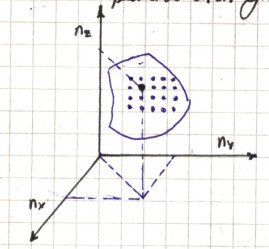
\includegraphics[width=0.4\textwidth]{images/fig_ft2_scattering_section_2.jpg}

Esta es la probabilidad de transición entre los impulsos $\vb{k}$, $\vb{k}'$. Es el número de partículas en 
la unidad de tiempo por unidad de área (ángulo sólido).
Definiremos la sección eficaz como:
\[
	\text{seccion eficaz} \equiv \dtot{\sigma}{\Omega}d\Omega =
	\frac{\text{\# de part en $d\Omega$ en la unidad de t}}
	{\text{\# de part incidentes en la unidad de t por unidad de área}}
\]

Para nuestra mecánica cuántica
\[
	\dtot{\sigma}{\Omega}d\Omega \equiv \frac{\omega_{k \to k'}}{\text{ flujo }}
\]
donde el flujo está relacionado con la expresión vista en física moderna, si
\[
	\Psi = \frac{ \euler^{ i \pe{k}{x} } }{ \sqrt{ L^3 } } \qquad \qquad 
	| \vb j | =  \left| \frac{\hbar}{m} \mathfrak{Im}( \Psi^* \nabla \Psi ) \right|
\]
donde este $|\vb j| = \hbar k $ m$^{-1}$L$^{-3}$ (cálculo con los dedos) pués flujo es velocidad sobre volumen.

Faltaría hallar quién es el elemento de matriz involucrado. Pensemos en un $V(\vb x)$ como caso particular.
Un elemento de matriz $\Braket{k'|V|k}$ será 
\[
	\Braket{\vb{k}'|V|\vb{k}} = \int dx'\Braket{\vb{k}'|\vb{x}'} \Braket{\vb{x}'|V|\vb{k}} =
	\int d\vb{x}' \frac{1}{L^3} \euler^{i (\vb{k}-\vb{k}')\cdot \vb{x}} \; V(\vb{x}'),
\]
con lo cual terminaríamos resolviendo una transformada de Fourier.
La transformada de Fourier del potencial es, amén de constantes, la amplitud a primer orden 
\[
	|\vb{k} - \vb{k}'| = 2k\sin(\theta/2) \qquad \text{con} \; k=k' 
\]
Entonces para cualquier potencial esféricamente simétrico se puede hacer la integral 
\[
	\dtot{\sigma}{\Omega} =
	\left|\left( \frac{2m}{4\pi\hbar}\right)^2 \int d^3x'\;V(x) \euler^{i(\vb{k}-\vb{k}')\cdot\vb{x}'}\right|^2
\]
y expresamos todo en función de $q=q(\theta)$
\[
	\dtot{\sigma}{\Omega} =
	\left| -\frac{2m}{\hbar^2} \frac{1}{q} \int_0^\infty rV(r)\sin(q) dr \right|^2.
\]

Este resultado es a primer orden (Born) y la dependencia de la sección eficaz está relacionada con el término
a primer orden del potencial.

Para el potencial de Coulomb diverge por el alcance infinito de éste. Por ello se suele utilizar otro tipo de
potenciales, como el de Yukawa,
\[
	V(r) = \frac{V_0}{r} \euler^{-\mu r} \qquad \qquad r \gg \frac{1}{\mu} \quad V \to 0
\]
este tiene la gracia de morirse más rápidamente que el de Coulomb. Definamos
\[
	\mathcal{F}_{kk'} = \Frac{2m}{4\pi\hbar^2}^2 \int d^3x \: V(x) \: \euler^{i(\vb{k}-\vb{k}')\cdot\vb{x}'}
\]
Se puede ver que 
\[
	\mathcal{F}_{kk'} = \mathcal{F}(\theta),
\]
que responde al esquema de abajo.
\includegraphics[width=0.5\textwidth]{images/teo2_31.pdf}	
Luego, como $\vb q = \vb{k} - \vb{k}'$
\[
	q = | \vb{k} - \vb{k}' | = 2 \: k \: \sin\left( \theta / 2 \right) \equiv q_r
\]
donde $\vb q$ es el desvío entre los momentos. Luego puedo realizar la integral fácilmente para
cualquier potencial simétricamente esférico.
\be
	 \mathcal{F}(\theta) = - \frac{2 m }{\hbar^2} \frac{1}{q}
	 \int_0^\infty \: r \: V(r) \: \sin( q_r ) \: dr 
	 \label{f_theta}
\ee
\be
	 \mathcal{F}(\theta) = - \frac{2 m V_0 }{ \hbar^2 } \frac{1}{q^2 + \mu^2}
	 \label{f_theta_2}
\ee
\notamargen{Esto es un mix.}
Nótese que metiendo $V(r)$ Coulomb aquí la integración \eqref{f_theta} no está bien definida.
En \eqref{f_theta_2} podemos tomar el límite que equivale a poner $V(r) = e^2/r$ (Coulomb), entonces
\[
	\mu \to 0, V_0 = e^2, \qquad \to \qquad 
	\mathcal{F}(\theta) \to - \frac{2 m e^2 }{ \hbar^2 } \frac{1}{ q^2 }
\]
Luego, la sección eficaz de Rutherford será
\[
	\dtot{\sigma}{\Omega} = \frac{ 2 m^2 e^4 }{ \hbar^4 } \frac{1}{ 16 k^4 \sin^4 (\theta / 2 ) }
\]
donde hemos detener en cuenta que la aproximación vale para un centro dispersor que no se mueve, mientras
todo el impulso cambia en las partículas bombardeantes. No vale si las masas son iguales.
Rutherford obtuvo este resultado en términos de energía
\[
	\dtot{\sigma}{\Omega} =  \frac{ e^4 }{ 16 E^2 \sin^4 (\theta / 2 ) }
\]
Este cálculo da lo mismo que en mecánica clásica de casualidad.

Utilizando un potencial de Yukawa primero y tomando el límite para llegar al de Coulomb tenemos la sección 
eficaz de Rutherford 
\[
	\dtot{\sigma}{\Omega} = \frac{2m^2e^4}{\hbar^4}\frac{1}{16k^4\sin^4(\theta/2)}
\]

hay que tomar el potencial de Yukawa y luego el límite porque el de Coulomb diverge de entrada

\subsection{Scattering con una distribución de cargas}

Ahora consideramos interacción no con un núcleo sino con una distribución normalizada
\[
	\int \: \rho(\vb x') \: d^3x' = 1
\]
y entonces
\[
	\frac{e^2}{r} \longrightarrow e^2 \int \frac{\rho(x')}{|\vb x - \vb x'|} d^3x'
\]

Ahora la sección eficaz dependerá de la distribución de cargas de forma que
\[
	\frac{ 2 m }{ 4 \pi \hbar^2 } e^2 \int d^3x \int d^3x' 
	\frac{ \rho(\vbx') \euler^{ i \pe{q}{x} } }{|\vbx - \vbx'|} = \dtot{\sigma}{\Omega}
\]
tomando el cambio de variables $\vb x \to \vb x + \vb x'$ será
\[
	\dtot{\sigma}{\Omega} = \frac{2 m e^2}{ 4 \pi \hbar^2} \left[ \int d^3x' \rho(\vbx') \euler^{i \pe{q}{x'}} \right] 
	\int d^3x \frac{\euler^{i \pe{q}{x}}}{r} = \frac{ 2 m e^2 }{\hbar^2 q^2} F(q)
\]
\notamargen{Es $4\pi/q^2$ es transformada de Fourier.}
donde $F(q)$ es el factor de forma (entre corchetes) y pudimos separar la sección eficaz en dos transformadas
de Fourier.
Luego,
\[
	\left. \dtot{\sigma}{\Omega} \right|_{\text{dist. carga}} = 
	\left. \dtot{\sigma}{\Omega} \right|_{\text{dist. carga}} |F(q)|^2
\]
el factor de forma nos da idea de la distribución de carga.

Podríamos pensar diagramáticamente la interacción como
	
	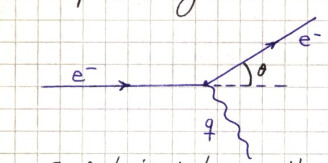
\includegraphics[width=0.5\textwidth]{images/fig_ft2_scattering_section_3.jpg}
	
donde el fotón tiene un impulso $q$ que es el que se intercambia con el blanco.
Podemos establecer un criterio de ``resolución'' como en óptica.
\begin{eqnarray*}
1 \text{eV} & 10^{-8} \; \text{ m}  \\
1 \text{KeV} & 10^{-11} \; \text{ m}  \\
1 \text{MeV} & 10^{-14} \; \text{ m}  \sim 10 \text{ Fermi } \\
1 \text{GeV} & 10^{-17} \; \text{ m}  
\end{eqnarray*}

La energía de lo incidente permite resolver detalles de la estructura atómica.
Entonces, para estudiar partículas con estructura del orden de $10^{-18}$ m ($e^-$, quarks)
necesitamos impactar con energías del orden de GeV (de ahí la necesidad de aceleradores de puta madre).


\begin{ejemplo}{\bf Ejercicio 16}
 
Parte a) 
Se tiene la situación siguiente
\[
	E_1 < E_2 \qquad \qquad 
	H_0 = E_1 \KB{1}{1} + E_2 \KB{2}{2}, \quad V_{11} = V_{22} = 0
\]
y además $V_{12} = V_{21}^* = \gamma \euler^{ i \omega t }$ con $\gamma \in \mathbb{R}$,
de manera que hay posibilidad de que transicione $\Ket{1} \to \Ket{2}$ dado
que $C_1(0)=1$ y $C_2(0)=0$.

Las probabilidades de transición serán $|C_i(t)|^2$ con $i=1,2$. 
El sistema (que será de $2\times 2$) para los coeficientes
\[
	i \hbar \begin{pmatrix}
	 \dot{C}_1 \\
	 \dot{C}_2 
	\end{pmatrix} = \begin{pmatrix}
	 V_{11} & V_{12} \euler^{ i \omega_{12} t } \\
	 V_{21} \euler^{i \omega_{21} t} & V_{22} 
	\end{pmatrix} \begin{pmatrix}
	 {C}_1 \\
	 {C}_2 
	\end{pmatrix} 
\]
\notamargen{En la carpeta tenía un sistema de tamaño genérico, aunque es un
caso de 2 por 2 aquí. No sé qué conviene más a esta altura.}
desde donde extraemos dos ecuaciones diferenciales acopladas
\[
	i \hbar \dtot{C_k}{t} = \sum_{n=1}^2
	V_{kn}(t) \: \euler^{ i \omega_{kn} t } \: C_n
\]
donde son 
\[
	\omega_{12} = \frac{E_1 - E_2}{\hbar}
	\qquad 
	-\omega_{12} = \omega_{21} = \frac{E_2 - E_1}{\hbar}
\]
tras lo cual se pueden escribir
\[
	i \hbar \dot{C}_1 = \gamma \euler^{i\Delta\omega t} C_2 
	\qquad 
	i \hbar \dot{C}_2 = \gamma \euler^{-i\Delta\omega t} C_1
\]
donde se ha definido $ \omega - \omega_{21} \equiv \Delta\omega$
y para la derivada segunda,
\[
	i \hbar \ddot{C}_1 = i \gamma \Delta\omega \euler^{i\Delta\omega t} C_2 +
	\gamma \euler^{i\Delta\omega t} \dot{C}_2
\]
Reemplazando $C_2, \dot{C}_2$ en función de $C_1, \dot{C}_1$ llegamos a
\[
	\ddot{C}_1 - i \Delta\omega \dot{C}_1 + \frac{\gamma^2}{\hbar^2} C_1 = 0,
\]
para la cual se propone una solución del tipo $C_1(t) = \euler^{\Gamma t}$
que resulta ser 
\[
	\Gamma =  i \frac{\Delta\omega}{2} \pm i 
	\sqrt{ \frac{\Delta\omega^2}{4} + \frac{\gamma^2}{\hbar^2} }
	= i \left( \frac{\Delta\omega}{2} \pm k \right)
\]
donde hemos definido $ k = \sqrt{ \Delta\omega^2 / 4 + \gamma^2 / \hbar^2 }$,
de modo que la solución general es
\[
	C_1(t) = A \euler^{ i (\Delta\omega/2 + k ) t  } + B \euler^{ i (\Delta\omega/2 - k ) t}
\]
en la cual faltaría $C_2$ para la información de las condiciones iniciales.
Para $C_2$ se tiene
\[
	C_2(t) = \frac{i\hbar}{\gamma} \euler^{-i\Delta \omega t}
	\left[ 
	i (\Delta\omega/2 + k ) A \euler^{ i (\Delta\omega/2 + k ) t  } + 
	i (\Delta\omega/2 - k ) B \euler^{ i (\Delta\omega/2 - k ) t}
	\right]
\]
desde la cual podemos obtener finalmente, usando $C_1(0) = 1$ y $C_2(0) = 0$ con 
$A+B=1$ de manera que 
\[
	A = \frac{1}{2} - \frac{\Delta\omega}{4k}
	\qquad 
	B = \frac{1}{2} + \frac{\Delta\omega}{4k}
\]
que da las soluciones
\[
	C_1^{(1)}(t) = \euler^{ i \Delta\omega t / 2}
	\left[ \cos( k t ) - \frac{i \Delta\omega }{ 2 k } \sin( k t ) \right]
\]
\[
	C_2^{(1)}(t) = - \frac{i\gamma}{\hbar k} \euler^{-i \Delta\omega t / 2} \sin( kt )
\]
con el $k$ anteriormente definido, 
que da las probabilidades
\[
	|C_2^{(1)}(t)|^2 = \frac{\gamma^2}{\hbar^2 k^2} \sin^2( k t ),
	\qquad 
	|C_1^{(1)}(t)|^2 = 1 - |C_2^{(1)}(t)|^2
\]
y este es el cálculo exacto [qué significará esto].

La parte b) implica 
\[
	 C_1^{(1)}(t) = i \delta_{ni} - \frac{i}{\hbar}
	 \int_0^t dt' V_{ni}(t') \euler^{ i \omega_{ni} t'}
	 \qquad \qquad 
	 C_1^{(1)}(t) = 1
\]
\[
	C_2^{(1)}(t) = - \frac{i}{\hbar}
	 \int_0^t dt' V_{21}(t') \euler^{ i \omega_{21} t'} =
	 - \frac{i}{\hbar}
	 \int_0^t dt' \gamma \euler^{ - i \Delta\omega t'}
\]
y esta integral es
\[
	C_2^{(1)}(t) = \frac{\gamma}{\hbar\Delta\omega}
	[ \euler^{-i\Delta\omega} - 1 ]
\]


Entonces, calculando el valor absoluto al cuadrado se tiene 
\[
	|C_2^{(1)}(t)|^2 = \frac{2\gamma^2}{\hbar^2\Delta\omega^2}
	[ 1 - \cos(\Delta\omega t) ]
\]
donde lo último corresponde a una aproximación a orden uno de $\gamma$.

Veamos qué sucede en la expresión exacta, que tiene $\gamma$ a orden dos
(al cuadrado).
Tomando $ k \approx \Delta\omega/2$ con $\gamma \ll 1$ se tiene
\[
	|C_2(t)|^2 \approx \frac{4\gamma^2}{\hbar^2\Delta\omega^2}
	\sin^2\Frac{\Delta\omega t}{2}
\]
y expresando el seno en términos del coseno (quizás llamada a apéndice)
\[
	|C_2(t)|^2 = \frac{2\gamma^2}{\hbar^2\Delta\omega^2}
	[ 1 - \cos^2(\Delta \omega t)]
\]
por lo tanto a primer orden en $\gamma$ ambos coinciden. Siempre esto es válido
si $\Delta\omega \neq 0$, es decir que no me hallo en condiciones de
resonancia.
A $t$ fijo si hay resonancia tendremos un gráfico para 
$ 4 / (\Delta\omega^2 )\sin^2(\Delta\omega t/ 2)$
que es de la pinta del gráfico de abajo

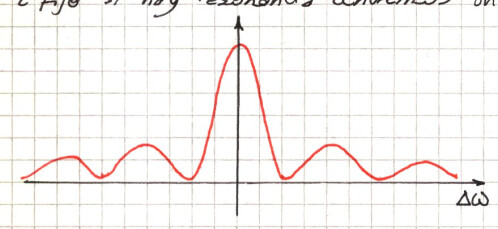
\includegraphics[width=0.5\textwidth]{images/fig_ft2_scattering_section_p1.jpg}

Si $\Delta \omega \to 0$ entonces
\[
	\lim_{\Delta \omega \to 0} \: \frac{\gamma^2}{\hbar^2}
	\frac{\sin^2(\Delta\omega/2 t)}{ (\Delta\omega)^2 / 4} =
	\frac{\gamma^2 t^2}{\hbar^2} = |C_2(t)|^2
\]

Volviendo ahora a la solución exacta tendremos 
\[
	|C_2(t)|^2 = \frac{\gamma^2}{\hbar^2 k^2}\sin^2( k t ) , 
	\qquad 
	k = \sqrt{ \frac{\Delta\omega^2}{4} + \frac{\gamma^2}{\hbar^2} } 
	= \frac{\gamma}{\hbar}
\]
que corresponde al caso resonante. Luego
\[
	|C_2(t)|^2 = \frac{\gamma^2}{\hbar^2 k^2}\sin^2\Frac{\gamma t}{\hbar} 
\]
y entonces $ |C_1(t)|^2 = 1 - |C_2(t)|^2 $.
Podemos graficar 

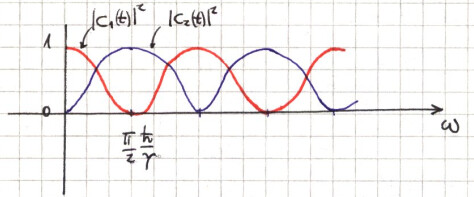
\includegraphics[width=0.5\textwidth]{images/fig_ft2_scattering_section_p2.jpg}
	
Vemos que está involucrado un $\Delta\omega = (E_2 - E_1)/\hbar$ de tal manera
que $\hbar\omega = E_2 - E_1$ es la energía que se absorbe o se libera para
pasar de estado. Ver grafiquete de abajo.
	
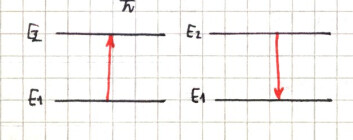
\includegraphics[width=0.5\textwidth]{images/fig_ft2_scattering_section_p3.jpg}


\end{ejemplo}


% \bibliographystyle{CBFT-apa-good}	% (uses file "apa-good.bst")
% \bibliography{CBFT.Referencias} % La base de datos bibliográfica

\end{document}
